\chapter*{Introduction}
\label{Introduction}
\addcontentsline{toc}{chapter}{\textbf{Introduction}}

%% Introduction large : 1-2 pages
Humanity is amidst a critical ecological era, whereby the limits of the earth system have been crossed. The notion of \textit{planetary boundaries} \citep{rockstrom2009safe,steffen_2015_planetary} illustrates how the anthroposphere, the planetary-scale effects of human activities, have become an additional functional component and capable of changing the Earth system \citep{richardson_earth_2023} alongside the goepshere (energy flow and nonliving materials in Earth and atmosphere) and biosphere (all living organisms/ecosystems). The \textit{planetary boundaries} framework identifies the limits to the impact of the anthroposphere on the Earth system that can safeguard Earth's interglacial state - the only one where civilization is known - by identifying a \textit{safe operating space}. The boundaries concern biosphere integrity, climate change, novel entities (e.g. man made introduction to the Earth system such as chemical and material pollutants), stratospheric ozone depletion, atmospheric aerosol loading, ocean acidication, biogeochemical flows, freshwater change and land system change. Among these 9 boundaries, \cite{richardson_earth_2023} estimate that 6 have been crossed, threatening the stability and resilience of the Earth system. 

\begin{figure}[H]
	\centering
	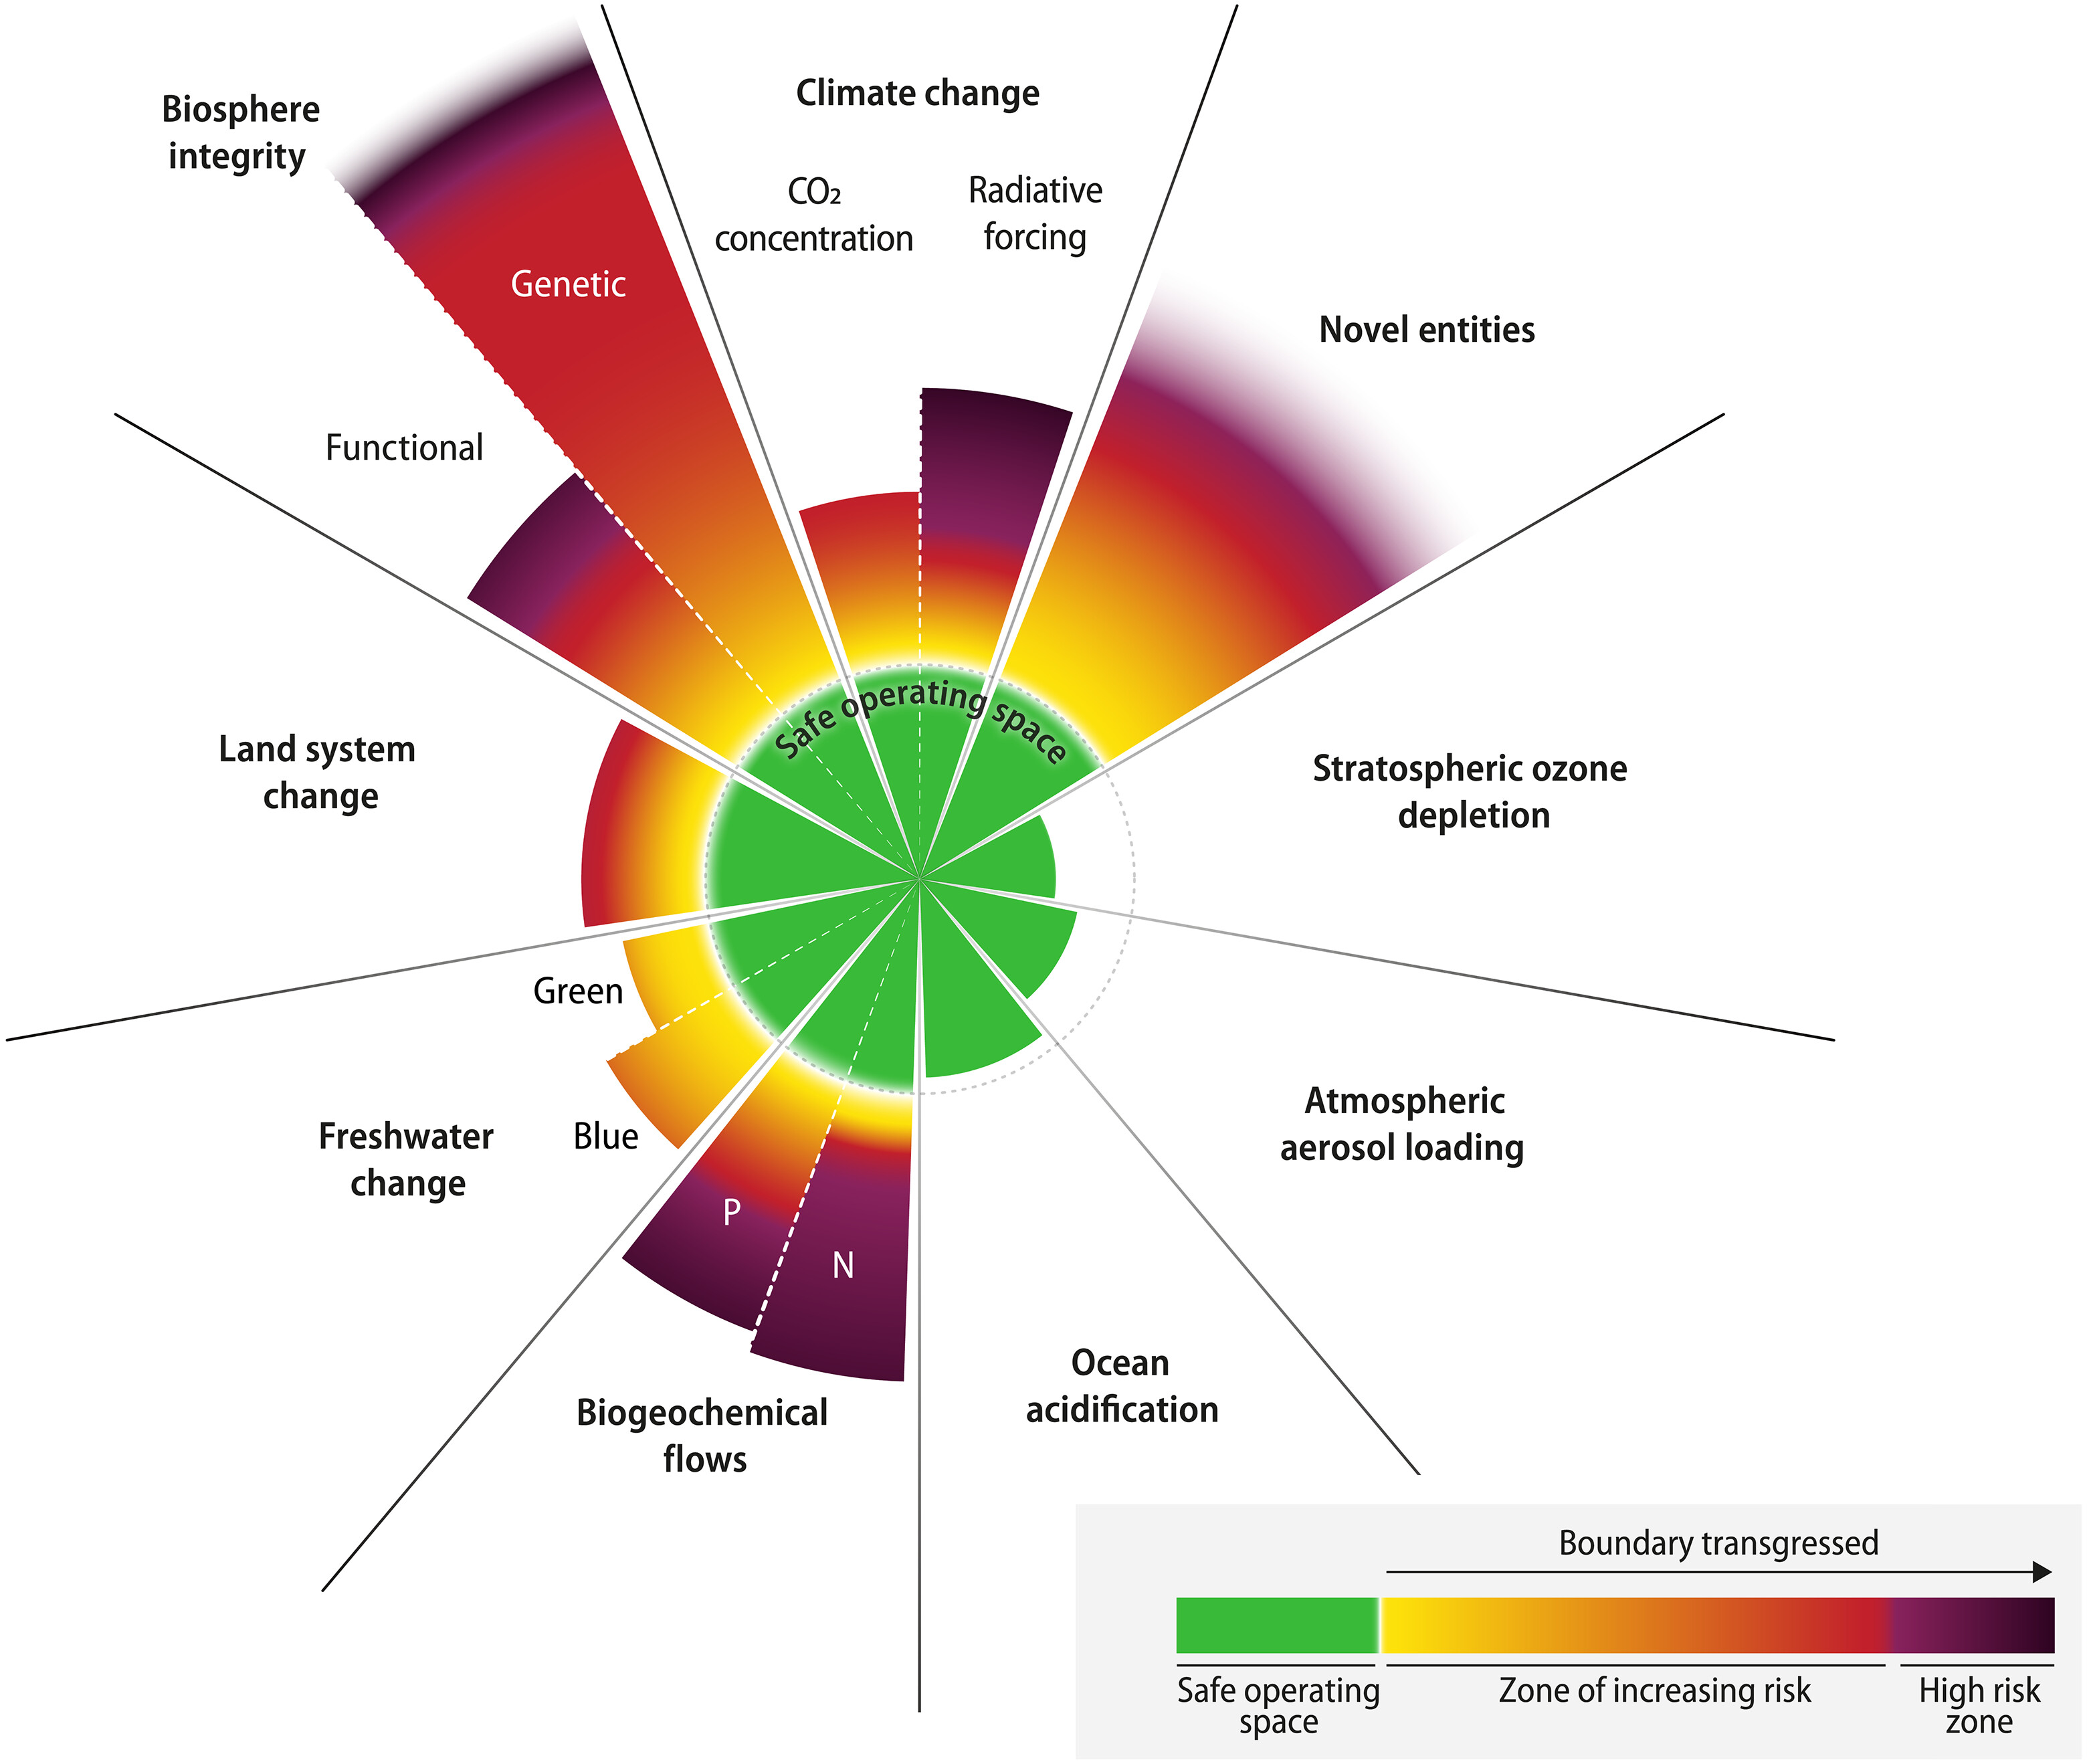
\includegraphics[width= .7\textwidth]{figures/intro/planetary_bounds.jpg}
	\caption{Current status of control variables for all nine planetary boundaries, from \cite{richardson_earth_2023}}
\end{figure}

Among these planetary limits, the integrity of the biosphere has gradually become of particular interest, along with its interaction with other limits, such as climate change, or novel entities (including pollution). Created in 2012, the Interdisciplinary Panel on Biodiversity and Ecosystem Services (IPBES) has been raising the alarm on the state of "Nature" globally. Its chair, Sir Robert Watson, put it clearly\footnote{See the \href{https://www.ipbes.net/news/Media-Release-Global-Assessment}{press release adress of the 2019 report}}:
\begin{displayquote}
"\textit{The overwhelming evidence of the IPBES Global Assessment\footnote{e.g. \cite{ipbes_2022_6417333}} from a wide range of different field of knowledge, presents an ominous picture [...]. The health of ecosystems on which we and other species depend is deterioritng more rapidly than ever. We are eroding the foundations of our economies, livelihoods, food security, health and quality of life worldwide}"
\end{displayquote}

The IPBES insists on four key elements about "Nature", a central concept in its framework \citep{ipbes_2022_6417333}:

\begin{displayquote}
\textit{Nature (also defined as living nature) [is] the nonhuman world, including coproduced features, with particular emphasis on living organisms, their diversity, their interactions among themselves, and with their abiotic environment. Within the framing of natural sciences, nature includes e.g. all dimensions of biodiversity, species, genotypes, populations, ecosystems, the biosphere, ecosystem functioning, communities, biomes, Earth life support's systems and their asosicated ecological, evolutionary, biogeochemical processes and biocultural diversity. Within the framework of economics, it includes categories such as biotic natural resources, natural capital, and natural assets. Within a wider context of social sciences and humanities and interdisciplinary environmental sciences, it is referred to with categories such as natural heritage, living environment, or the nonhuman. Within the context of other knowledge systems, it includes categories such as Mother Earth [...], Pachammama [...]} (\cite{ipbes_2022_6417333}, p.14, see also \cite{DIAZ20151})
\end{displayquote}


Nature, as defined in this approach, is a very large object. It is defined across different ontologies (living and non living) and types of interactions, at different scales (genotypes v. ecosystems), at different types of processes (biological v. ecological), and cross different fields of inquiry (natural sciences v. social sciences). 
In this dissertation, I study more specifically "biodiversity", which focuses on the variability among living organisms. While it is itself an ambiguous concept, biodiversity tends to isolates the functioning of living organisms, in relationship with their material, biotic and abiotic environemnt. Putting the focal on biodiversity allows to isolate 

First, it documents the drastic changes the biosphere is going through, how Nature and more specifically, biodiversity  is changing, across scales, time and geographic areas. Second, it mostly considers these changes through an \textit{anthropocentric} lense, e.g. mediating the aforementioned changes through the multiple and diverse contributions that Nature and biodiversity bring to people and how its disruption impacts human lives. Third, it highlights the role of anthropogenic (e.g. of human origin) drivers of the disruption of Nature and biodiversity. Finally, as it underpins ``\textit{our economies, livelihoods, food security health and qualitify of life worldwide}", the synthesis of the available science calls for collective action and suggests policy pathways to remedy the demise of Nature and biodiversity. 

 
This reports sets different objectives to scientific research. The first objective is to explain the feedback mechanisms : how do human livelihoods impact biodiversity? In response, how does biodiversity impact human livelihoods?. This objective involves understanding the causes and measuring the direct and indirect anthropogenic drivers of change in Nature and biodiversity on the one hand, and understanding the channels and scales through which Nature and biodiversity contribute to human livelihoods, as well as measuring these contributions. Hence, studying the demise of nature, and the potential to remedy it, calls for an integrated perspective, that joins natural sciences to social sciences, through frameworks such as \textit{social-ecological systems} \citep{Ostrom2009}. 
\\
The second objective is to provide a framework to assess the desirability, the feasibility and means of implementation of collective pathways that would remedy the crisis Nature is facing. In a way, it involves designing and implementing \textit{policy pathways} towards \textit{sustainable futures}, e.g. finding definite courses or methods of action selected from alternatives, at the individual, collective or governmental levels, to achieve future states of the world which remain in a safe operating space regarding planetary bounds \citep{rockstrom2009safe,steffen_2015_planetary}.


In this dissertation, I take on these two objectives using a framework stemming from economics and ecology. I study the feedback relationship between biodiversity and anthropogenic drivers of its decline, through their causes and consequences, and I analyze policy pathways to remedy this demise. 


\clearpage
\section*{The decline of Nature }
\addcontentsline{toc}{section}{The decline of Nature}

"Biodiversity" is also an ambiguous concept, which nonetheless has measurable features, which all point towards a marked decline attributable to mankind. Existing policy frameworks at different levels are geared to halt this decline. 


\subsection*{Emergence and definition of biodiversity as a concept}
\addcontentsline{toc}{subsection}{Emergence and definition of biodiversity as a concept}

Biodiversity emerged as a concept in the 1980s, along with the emergence of "conservation biology", a branch of biology concerned with the protection of "biological diversity" \citep{soule_what_1985}, as a response to an acceleration in the loss of species  that have intrinsic value, e.g. should be protected for their own sake \citep{soule_conservation_1986}. As highlighted by \cite{mouysset_diversity_2023} and \cite{VanDyke2008}, the conceptual definition of biodiversity is difficult, as it recovers a number of different dimensions. As a matter of fact, it recovers ethical and measurement concerns. Biodiversity can be viewed as "an intrinsic, value-ladden quality of natural systems that should be preserved for its own sake" \citep{VanDyke2008, mouysset_diversity_2023}, but it also refers to measurable features relevant to understanding community structure, environmental processes, and ecosystem functions. Although measurable, these features are epistemologically distinct as they measure different types of phenomena. 

In the wake of the 1992 Rio United Conference on Environment and Development,  the Convention on Biological Diversity emerged as an international treaty to safeguard biodiversity. In doing so, it provided an internationally agreed upon definition:

\begin{displayquote}
"\textit{"Biological diversity" means the variability among living organisms from all sources including, inter alia, terrestrial, marine and other aquatic ecosystems and the ecological complexes of which they are part; this includes diversity within species, between species and of ecosystems.}"\\
\small{\href{https://www.cbd.int/convention/articles/default.shtml?a=cbd-02}{Article 2 of the Convention on Biological Diversity}}
\end{displayquote}

Following \cite{mouysset_diversity_2023}, this definition implies different scales from a hierarchical perspective, at the genetic level, at the species, the community (e.g assembly of interacting species in a given area), and the ecosystem levels (defined as the interaction of communities and their abiotic environment). These levels imply different forms of measurement, including the distribution of genes, species abundance (e.g. the number of individuals), species richness (e.g. the number of different species) within communities, among communities, and across larger scales (e.g. alpha, beta and gamma diversities.), as well as variations in the abiotic factors that form ecosystems, such as temperature, humidity, water quality, soil quality etc. 
\\
It also comprises different types of diversity : structural diversity (for example, the layers of canopy in forests, the sex-ratio in animal populations), compositional diversity (the variety and abundance of species within a community), and functional diversity (variety of environmental processes performed by living organisms in a given area e.g. carbon sequestration, nutrient cycling or seed dispersal). Second, structural diversity refers to the way elements are arranged within a group e.g. the layers of canopy in forests, the sex-ratio in animal populations. Finally, functional diversity is the variation of processes performed by elements within a group, e.g. carbon sequestration, nutrient cycling or seed dispersal.

\begin{figure}
	\centering
	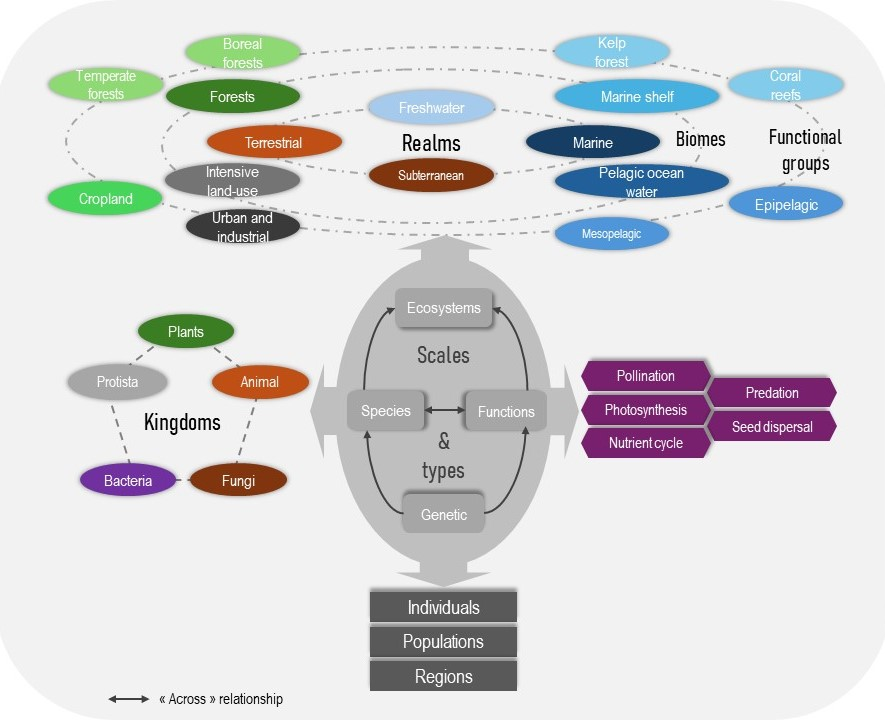
\includegraphics[width =.8\textwidth]{figures/intro/biodiv_illustration.jpg}
	\caption{Biodiversity : a multiform concept across scales and types}
	\label{fig:intro_biod}
\end{figure}

In this dissertation, I focus on the evolution of single species populations and on the evolution of communities  within a given ecosystem. Moreover, I study the importance of structural diversity at the species and community levels, and focus on animal species. 

\subsection*{Documenting the decline through different scales and types}
\addcontentsline{toc}{subsection}{Documenting the decline through scales}

There has been an ongoing decline in metrics surrounding biodiversity. Across all the scales of analysis, the state of nature is critical. The structural conditions of ecosystems (e.g. interactions between biotic and abiotic elements that cause different structural phenomena and lead ecosystems to provide various resources, including wildlife habitat, carbon sequestration etc), the compositions (e.g. species richness\footnote{ Species richness measures the \textit{number of species} in a given period and location}) of ecological communities and populations (e.g. species abundance\footnote{ Species abundance measures the \textit{population of species} in a given period and location}) of species have experienced dramatic changes. 

Ecosystem structure e.g. the arrangement of biotic and abiotic elements through time and space, forms the basis of natural and social-ecological processes. Ecosystems can be classified among realms (terrestrial, subterranean, marine, freshwater etc), biomes (e.g. forests, intensive land uses, marine shelf, pelagic ocean water) and functional groups (temperate forests, cropland, coral reefs, etc) (see figure \ref{fig:intro_biod}). Ecosystem characteristics are severely degraded: only 13\% of oceans and 23\% of land remains sufficiently unimpacted by humanity to be classified as \textit{wilderness} \citep{watson_2016_catastrophic, jones_2018_location}. e.g. areas with "biologically and ecologically largely intact landscapes that are mostly free of human disturbance". On land, at a more refined scale, while deforestation has slowed since the 1990s, vegetation biomass (including trees) has dropped to below 50\% of the level expected absent human land-use, suggesting that a planetary boundary has been crossed \citep{steffen_2015_planetary}. Additionally, anthropogenic climate change drives ecosystem disruptions on land \citep{burrell_anthropogenic_2020, conradi_reassessment_2024} and at sea \citep{gomes_marine_2024}, through changes in various channels including ecological suitability and foodweb disturbances.

Community compositions are changing rapidly, but the average effect remains unclear, as the introduction of alien, disturbance tolerant, climate-migrant species faces local extinctions is spatially hetorogeneous \citep{cardinale_local_2018}. Analysis from long series of spatial data show contrasted results, because of geographic biases, on land and at sea \citep{dornelas_assemblage_2014, gonzales_estimating_2016}. When taking a historical reference point, however, the fraction of originally present biodiversity falls well below 90\% across all biomes \citep{Hill311787}. Nonetheless, it appears that local communities are becoming more and more similar \citep{mckinney_1999_biotic}, driven by the increased extent of animal and plant non-alien invasive species, rising by 13\% per decade \citep{seebens_no_2017}. 
On aggregate, species richness per grid cell is difficult to measure, as slight decreases measured since 1970 \citep{Kim300632} do not account for species introduction, nor potentially unredeemed extinction debts (see below) \citep{JACKSON2010153}.

Finally, at the species level, global species richness is  threatened by a mass extinction, as the global rate of species extinction is at least ten times higher than the average rate over the past 10 million years and is accelerating \citep{barnosky_has_2011, ceballos_accelerated_2015}. On average, 25\% of species are currently threatened with global extinction (Figure \ref{fig:intro_iucn}, \cite{IUCN_redlist_2024}) across a wide range of plant and animal species, on land and at sea. Using different methods\footnote{ The IUCN Redlist uses detailed accounts for species, in a bottom-up approach, to analyze the extinction risk of species. A top-down approach, relying on the evolution of available habitat and the species-area relationship, uses changes in land use to forecast the extinction of species in a more aggregate manner \citep{Diamond1972BiogeographicKE}}, \cite{Hoskins309377} find that hundreds of thousands of plant and animal species are threatened, and will repay the \textit{extinction debt} caused by anthropogenic changes to their habitats : only 92.1\% of terrestrial vertebrate species, 91.6\% of terrestiral invertebrates and 90.7\% of terrestrial plants have enough habitat to persist. These results suggest that around half a million terrestrial animal and plant species - including over 3000 vertebrates and over 40,000 plants - \textit{dead species walking}, doomed to become extinct, unless their habitats improve in time to prevent it \citep{ipbes_2022_6417333}.

\begin{figure}[h]
    \centering
    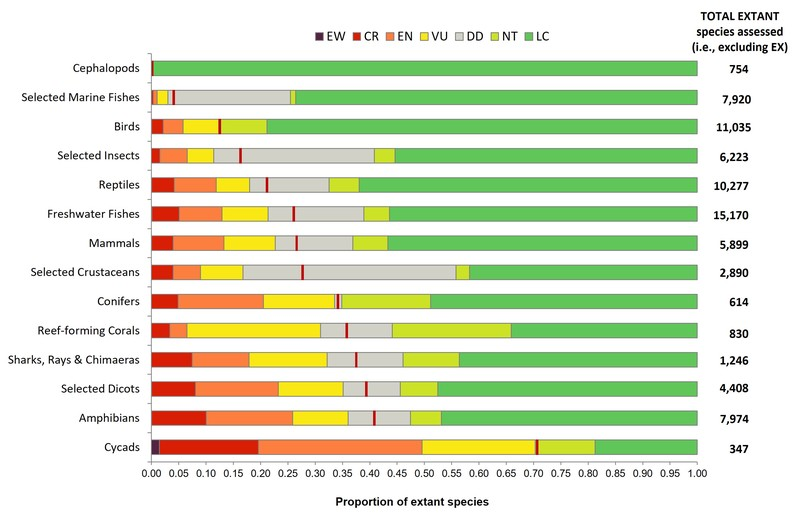
\includegraphics[width=0.8\linewidth]{figures/intro/IUCN_redlist}
    \caption{The proportion of extant (i.e., excluding Extinct) species in \citet{IUCN_redlist_2024}}
    \subcaption*{Assessed in each category for the more comprehensively assessed (i.e., at least 80\% of the group has been assessed) groups containing $\geq$ 150 species. Species are grouped into classes. The numbers to the right of each bar represent the total number of extant species assessed for each group. \textbf{EW} - Extinct in the Wild, \textbf{CR} - Critically Endangered,\textbf{ EN} - Endangered, \textbf{VU} - Vulnerable, \textbf{NT} - Near Threatened, \textbf{DD} - Data Deficient, \textbf{LC} - Least Concern.}
    \label{fig:intro_iucn}
\end{figure}

The concept of biodiversity was forged to highlight the need to safeguard the diversity of living organisms across scales from an extinction crisis, acknowledging the threat is first and foremost human. 

\subsection*{Anthropogenic drivers of biodiversity decline}
\addcontentsline{toc}{subsection}{Anthropogenic drivers of biodiversity decline}

The drivers of biodiversity decline are of anthropogenic source. They can be classified between \textit{direct} drivers, e.g. that directly flow form human actions, such as land use change, anthropogenic climate change, overexploitation, and \textit{indirect} drivers, that can be viewed as the root cause for direct drivers, such as  , changes in the value systems that underpin nature uses (\cite{ipbes_2022_6417333} p.55), demography (urbanization and migration), technology, economy (sectoral transitions, trade expansion) and governance (including risht systems for access to resources).

The impact of direct drivers can be differentiated among terrestrial and marine species, as well among types of biomes.  Synthesis of the available science \citep{ipbes_2022_6417333} (section 2.2.6.2) show that land and sea use, reefering to the loss, fragmentation and degradation of wildlife habitat are responsible for 30\% of the impacts on biodiversity. The direct exploitation of wildlife, wild plants and trees represents 23\% of impacts. Climate change, through shifts in biogeographic conditions and changes in habit, impacts on species traits and genetic evolution represents 14\%, and pollution represents 14\% of impacts. Finally invasive alien species represent 11\%. These drivers have differenciated impacts across ecosystems and biomes \citep{ipbes_2022_6417333}. 
% Forests

For terrestrial species, land use change is the most important driver (30.5\%), driven by deforestation and agriculture, and direct exploitation follows next (21\%). 
Tropical and subtropical dry and humid forest host the greatest biological diversity. For example, they host the 10 hotspots with the greatest total number of vertebrates \citep{mittermeier_global_2011}. In such forests, habitat loss and degradation are the main drivers of reductions in species abundance and richness \citep{newbold_global_2014}. Legal and illegal selective logging destroy habitat \citep{hoare2022establishing,  bousfield_2023_large} and are combined with hunting and poaching of wildlife \citep{gallego_2020_combined}, 
%generating between 60 and 180  billions  \$ USD of revenue \citep{gfi_2017}\footnote{Illegal wildlife trade represents between 5 and 23 billion \$USD, while illegal logging represents 52 to 157 billion \$USD}.
 Mediterranean forests, wooldlands and scrubs, covering 4 million km$^2$, are areas of exceptionally high diversity too \citep{Mooney2001, blondel_2010}. However, they are faced with a conjunction of threats, including climate change, land-use transformations \citep{newbold_tropical_2020} and wildfires \citep{Dupuy2019ClimateCI}. Indeed, wildfire frequency and severity are expected to increase with global warming, causing important direct and indirect costs to society including destruction of infrastructure and perturbations to economic activity \citep{wang_economic_2021}, smoke related health conditions \citep{burke_wildfire_2023, heft-neal_behavior_2023}, disrupting structural features of ecosystems \citep{Ayars2023} and threatening biological diversity \citep{Wintle2020}.
% Oceans and fish

For marine species, overexploitation is the main driver (29\%) \citep{ipbes_2022_6417333}. With 90 million tons of capture 
%(and 141 billion \$ USD) 
in 2020 \citep{fao_2022_state}, fisheries stock within biologically sustainable levels have decreased to 64.6\% in 2019, from 90\% in 1974\footnote{ In this calculation, all fishery stocks are equally counted, irrespective of their abundance or catch}, driven by overfishing in the Southeast Pacific and the Mediterranean and Black seas. Assessment of fisheries stock and catch management have been proved to improve livelihoods as well as fish stocks globally \citep{melnychuk_2017_fisheries, hilborn_2020_effective}. Nonetheless, illegal, unreported and unregulated (IUU) fishing is a threat to fisheries. Estimates from 15 years ago \citep{agnew_estimating_2009} estimated it represented between 11 and 26 million tonnes of fish.
% with a value of 10 to 23 billion \$ USD. 
It typically arises in weak governance contexts, with high economic incentives and barriers to enforcement \citep{iuu_2020_widjaja}. 


\section*{The Importance of Biodiversity and the Challenges of Conservation}
\addcontentsline{toc}{section}{The Importance of Biodiversity and the Challenges of Conservation}



\subsection*{Nature's Contributions to People should be protected}
\addcontentsline{toc}{subsection}{Nature's Contributions to People should be protected}



NCPs
Need for action
Weak substitutability and call for action

\subsection*{Adressing the drivers of decline}
\addcontentsline{toc}{subsection}{Adressing the drivers of decline}
Pas oublier la conjonction des effets e.g. land and climate change and effects aggregated
\subsection*{Policies for remedying the decline}
\addcontentsline{toc}{subsection}{Policies for remedying the decline}


\section*{From the economy to the economics of biodiversity}
\addcontentsline{toc}{section}{From the economy to the economics of biodiversity}
\subsection*{Biodiversity as an economic object}
\addcontentsline{toc}{subsection}{Biodiversity as an economic object}

\subsection*{How to do the economics of biodiversity? Choice of method}
\addcontentsline{toc}{subsection}{How to do the economics of biodiversity? Choice of method}

\subsection*{Specific bioeconomic modeling challenges in the face of anthropogenic drivers}
\addcontentsline{toc}{subsection}{Specific bioeconomic modeling challenges in the face of anthropogenic drivers}



\section*{Dissertation outline}
\addcontentsline{toc}{section}{Dissertation outline}







%% Global biodiversity decline : why should we care?

%% Conceptual challenges



